\documentclass[twocolumn]{article}
\usepackage{caption}
\usepackage[utf8]{inputenc}
\usepackage{amsmath}
\usepackage[margin=1in]{geometry}
\usepackage{changepage}
\usepackage{titling}
\usepackage{ragged2e}
\usepackage{abstract}
\usepackage{enumitem}
\usepackage{graphicx}
\usepackage{hyperref}
\renewcommand{\thesection}{\Roman{section}.}
\renewcommand{\thesubsection}{(\roman{subsection})}
\renewcommand{\thesubsubsection}{\thesubsection.\alph{subsubsection}}
\setlength\parindent{5pt}
\setlength{\columnsep}{1cm}

\begin{document}

\twocolumn[
\begin{@twocolumnfalse}
\title{\Large{\textbf{Optical Pumping of $Rb^{85}$ and $Rb^{87}$}}}
\author{Herbert D. Ludowieg}
\setlength{\droptitle}{-0.65in}
\maketitle
\begin{onecolabstract}
\justify
Optical Pumping is a spectroscopical method that was developed in the 1950's 
and has been a very accurate method to determine spectroscopical properties of 
certain materials. In this experiment the following were determined: the 
individual g-factors, nuclear spins, cross sectional area and ratio of the 
periods. For $Rb^{85}$ the g-factor and nuclear spin were found to be: 
0.3260 $\pm$ 0.0005 and 2.571 respectively. For $Rb^{87}$ they were found to 
be: 0.482 $\pm$ 0.001 and 1.576 respectively. The cross-sectional area and 
ratio of the periods were found to be: 1.8$\times10^{-16}$ $\pm$ 
0.3$\times10^{-16}$ and 1.44 $\pm$ 0.05 respectively.
\\
\end{onecolabstract}
\end{@twocolumnfalse}]

\section{Introduction}
Optical Pumping is a spectroscopical method developed in 1950 by Alfred 
Kastler, whom received the Nobel Prize in physics in 1966 for his discovery. 
This method is one in which photons are utilized to create population 
differences of electronic excited and ground states. So the meaning and general 
concept is in the name itself.
\\
Under startdard conditions the population difference required to carry out 
experiments is not possible because from statistical mechanics at thermal 
equilibrium we have an equal number of electrons that rise and fall from 
excitation levels. Due to this, they tend to cancel each others effects and 
no net population differences can be detected. This is also the basis of lasers 
where, a population difference needs to be created so that photons can be 
spontaneously emmitted by the lasing medium.
\\
For this experiment the equipment that is being used is provided by TeachSpin 
and consists of an Radio Frequency (RF) discharge lamp, Interference Filter, 
Polarizers, Quarter Wave plate, absorption cell, optical detector, three sets 
of magnetic coils in a Helmholtz configuration and a RF magnetic coil. The 
sample is a rubidium glass bulb that contains neon gas with a pressure of 
approximately 0.04 atm pressure. The presence of the neon gas is important as 
its spherical symmetry will reduce the interactions between the rubidium atoms 
and the outside environment. They will act as a buffer gas.
\\
Optical Pumping is a process in which has had much applicability in solid state 
and liquid state physics. However, we will only be dealing with a gas since at 
the solid and liquid phases the interactions between the neighboring atoms 
increases thus broadening the energy levels \cite{ref:1}.

\section{Theory}
\subsection{Structure of alkali atoms}
\begin{figure*}
\center
\begin{minipage}{0.45\linewidth}
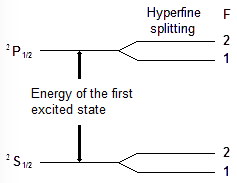
\includegraphics[width=\linewidth]{pictures/hyperfine-splitting.png}
\caption{\textit{Hyperfine splitting energy diagram for I = 3/2 particle
\cite{ref:3}}}
\label{fig:3}
\end{minipage}
\hfill
\begin{minipage}{0.45\linewidth}
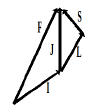
\includegraphics[width=0.3\linewidth]{pictures/hyperfine-vectors.png}
\caption{\textit{Hyperfine coupling in an alkali atom \cite{ref:3}}}
\label{fig:4}
\end{minipage}
\end{figure*}
In the experiment described in this paper we will be studying the absorption 
and emission from rubidium isotopes (85 and 87) which are alkali atoms. As such the electronic structure of rubidium is as such,
\begin{equation*}
1s^22s^22p^63s^23p^63d^104s^24p^65s
\end{equation*}
Where we can show the shorthand version as,
\begin{equation*}
[Kr]5s
\end{equation*}
\center
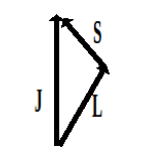
\includegraphics[width=0.3\linewidth]{pictures/electron-angular-momentum.png}
\captionof{figure}{\textit{Coupling of angular momentum in an electron 
\cite{ref:3}.\\}}
\label{fig:1}
\justify
Where, the superscripts show the number of electrons contained in each of the 
electronic shells. Since the only valence electron is in the 5s shell we can 
consider the atom to bev consisting of only one electron. This electron much 
like with other 
electrons can be described by means of the total angular momentum of the 
electron $\vec{J}$ where it is made up of components $\vec{S}$ and 
$\vec{L}$. Which, represent the spin angular momentum and orbital angular 
momentum respectively. The vectors are shown on figure \ref{fig:1}
\\
Since, these components are vectors we can represent the total angular momentum 
as such,
\begin{equation}
\vec{J} = \vec{S}+\vec{L}
\label{eqn:1}
\end{equation}
\justify
Where, for an alkali atom in the ground state the value of $\vec{L}$ is zero 
from the quantum numbers associated with the orbital shell and the value of 
$\vec{S}$ will be 1/2. So, this gives rise to a total angular momentum of 1/2.
\\
As it will later become apparent, we will display some of the energy levels in 
the notation $^{2s+1}L_J$. Where, all of the values are those taken from 
equation \ref{eqn:1}. To represent the ground state of an alkali atom we can 
write it with the formatting $^{2}S_{1/2}$. Since the value of $\vec{L}$ is 
zero by convention we write it as the letter S. Where it to be 1 we would write 
in P and so on.
\\
If the electron were to be in a P state it would be able to have an angular 
momentum of $\vec{L}\pm\vec{S}$ and would take on the representations 
$^{2}P_{1/2}$ and $^{2}P_{3/2}$. Due to the difference in angular momentum the 
energy levels would have different energies. This arises due to the spin-orbit 
coupling of the angular momentum vectors \cite{ref:4}.
\center
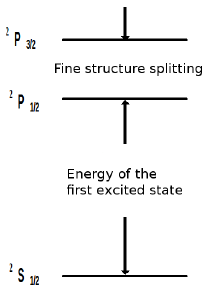
\includegraphics[width=0.5\linewidth]{pictures/energy-levels.png}
\captionof{figure}{\textit{Pictoral representation of the energy difference in the fine structure. Not to scale \cite{ref:3}.}}
\label{fig:2}
\justify
So far, we have been ignoring the effects of the nucleus to make the theory 
easier. However, this will not go on any longer. We will now consider the 
hyperfine splitting of the electron angular momenta. This arises from the 
spin-spin coupling where for the fine structure we had the spin-orbit coupling. 
\\
The spin-spin coupling is due to the magnetic dipole moment of both the proton 
and electron. Now, it should be noted, that the magnetic dipole moment of the 
proton is much smaller than that compared to the electron. The dipole momenta 
can be given as the following.
\begin{equation}
\begin{aligned}
\vec{\mu_p} &= \frac{g_pe}{2m_p}\vec{S_p}
\qquad
\vec{\mu_e} &= -\frac{e}{m_e}\vec{S_e}
\label{eqn:2}
\cite{ref:4}
\end{aligned}
\end{equation}
Where, the p and e represent the proton and electron values respectively, $g_p$ and $g_e$ are the respective g-factors of value 5.59 and 2.00 and $\vec{S}$ 
represents the respective angular spin. Using derivations outlined in reference 
\cite{ref:4} we can get to an expression for the difference in energy of the 
two states with different angular momenta. The equation is as such.
\begin{equation}
\Delta E = \frac{4g_p\hbar}{3m_pm_e^2c^2r^4}
\label{eqn:3}
\cite{ref:4}
\end{equation}
Where, c is the speed of light and r is the radius of the atom. In the 
reference they are making an example to a hydrogen atom with r equal to a 
(Bohr's atomic radius). This derivation can still be generalized to our use as 
we are dealing with an atom that can be approximated to be one that is like a 
hydrogen atom, due to the closed nature of the inner shells. 
Where we can also make the relation with the frequency as such.
\begin{equation}
\nu = \frac{\Delta E}{h}
\label{eqn:4}
\cite{ref:4}
\end{equation}
Where the Hamiltonian is as such.
\begin{equation}
H=ha\vec{I}\cdot\vec{J}
\label{eqn:5}
\cite{ref:3}
\end{equation}
Usually the energy difference between these two levels is very small and one 
can cause transitions in the hyperfine structure with an RF wave. A pictoral 
representation of the coupling of the magnetic dipole moment spins is shown on 
figure \ref{fig:4}. Where a rough enegy separation schematic is given in figure 
\ref{fig:3}. As is clearly seen the energy that is required to jump from one 
energy level to the next is much greater than that required to make the 
transition in the hyperfine structure. Later we will discuss the implications 
of this with respect to optical pumping.
\\
However next we will show another form of splitting where all of the degenerate 
energy levels of the electronic energy level diagram are split.

\subsection{Interaction of an alkali atom with a magnetic field}
\begin{figure*}
\center
\begin{minipage}{0.45\linewidth}
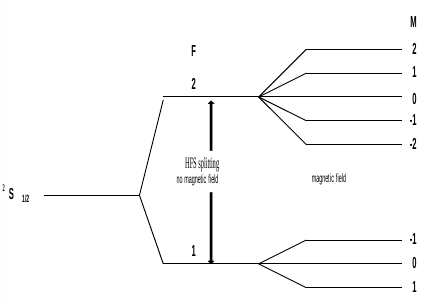
\includegraphics[width=\linewidth]{pictures/zeeman-splitting.png}
\caption{\textit{Energy levels of an alkali atom of the $^2S_{1/2}$ state in a 
weak magnetic field \cite{ref:3}}}
\label{fig:5}
\end{minipage}
\hfill
\begin{minipage}{0.45\linewidth}
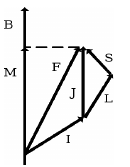
\includegraphics[width=0.3\linewidth]{pictures/zeeman-vectors.png}
\caption{\textit{Zeeman effect in an alkali atom \cite{ref:3}}}
\label{fig:6}
\end{minipage}
\end{figure*}
This interaction is better known as the Zeeman effect and the general premise 
behind this effect is that by applying a magnetic field to an atom we can 
further split the degenerate energy levels according to their angular momenta.
\\
In the Zeeman effect there are three main regions that are to be considered: 
weak field, intermediate and Strong field effects. For the purposes of this 
experiment we will only deal with the weak field effect as the strong field 
can require magnetic fields around 10T which is only achievable with 
extremely expensive equipment.
\\
The Zeeman effect is an effect which can break the spin-orbit coupling of an 
electron creating a difference in energy between the different orbitals of an 
atom. The weak field Zeeman effect is named as such because the energy 
splitting from the Zeeman effect is very small comparatively and as such the 
Hyperfine splittings dominate with the Zeeman effect becoming the pertubation 
\cite{ref:4}. The hamiltonian of this effect is as shown.
\begin{equation}
H=ha\vec{I}\cdot\vec{J}-\frac{\mu_J}{J}\vec{J}\cdot\vec{B}-\frac{\mu_I}{I}\vec{I}\cdot{B}
\label{eqn:6}
\cite{ref:3}
\end{equation}
Where, $\mu_J$ is the electronic dipole moment and $\mu_I$ is the nuclear 
magnetic dipole moment.
\\
Figure \ref{fig:5} shows the energy levels from the weak field Zeeman effect. 
The energy levels are splitting into $2F+1$ levels. Where F is the angular 
momentum of the atom, M is the projection of F onto the direction of the 
magnetic field. In figure \ref{fig:1} we show two levels for the ground state 
and the first excited state. For this experiment we are only considering the 
first excited state $^2P_{1/2}$. The reason why we only consider this and not 
the $^2P_{3/2}$ is because at $\vec{J}$ values of 1/2 we can calculate the 
energy levels in closed form from quantum mechanics with the Breit-Rabi 
equation.
\\
Since the electron can be considered to be a moving charge with charge 1.6e-19 
Coulombs. This magnetic dipole moment has a value that is equal to the Bohr 
Magneton, $\mu_B$. Ignoring the effects of the nucleus we can then represent 
the magnetic energy as \cite{ref:3}.
\begin{equation}
U = \frac{M(\vec{L}+2\vec{S})\cdot\vec{J}}{J^2}\mu_B B = g_J\mu_B M B
\label{eqn:7}
\cite{ref:3}
\end{equation}
Where, $g_J$ is the Lande g-factor which describes the change in the magnetic 
moment of an electron bound in an atom, B is the magnetic field and M is the 
atomic spin component along the magnetic field direction. The g-factor is 
given by,
\begin{equation}
\begin{aligned}
g_J &= \frac{(\vec{L}+2\vec{S})\cdot\vec{J}}{J^2}
\\
g_J &= 1+\frac{J(J+1)+S(S+1)-L(L+1)}{2J(J+1)}
\label{eqn:8}
\cite{ref:3}
\end{aligned}
\end{equation}
To show the interaction energy of an electron we simply need to add a negative 
sign to equation \ref{eqn:7} from the negative charge of the electron. In the 
case of rubidium where we have a J and S value of 1/2 we find that the g-factor 
is equal to 2.00232 \cite{ref:3}.
\\
Now, if we were to include the interaction of the nucleus to find the 
interaction energy the equation could be represented as follows.
\begin{equation}
U = -g_F\mu_B M B
\label{eqn:9}
\cite{ref:3}
\end{equation}
Where, $g_F$ can be shown to be the following.
\begin{equation}
g_F = g_J\frac{F(F+1)+J(J+1)-I(I-1)}{2F(F+1)}
\label{eqn:10}
\cite{ref:3}
\end{equation}
Where, F represents the total angular momentum of the atom, I is the total 
nuclear spin angular momentum and J is the total electronic angular momentum. 
This quantity is highly dependent on the atom that is being used and as such 
there is no one set value as with the Lande g-factor.
\\
We can then show the transition frequency as.
\begin{equation}
\nu = \frac{g_F\mu_B B}{h}
\label{eqn:11}
\cite{ref:3}
\end{equation}
The above equations are only applicable when the interaction energy with the 
magnetic field is very small and depends linearly. If the dependence is 
quadratic, which will be studied in this experiment, we must apply the 
Breit-Rabi equation which can be derived by diagonalizing the Hamiltonian in 
equation \ref{eqn:6} \cite{ref:3}. The result of such is the following.
\begin{equation}
\begin{aligned}
W(F,&M) = -\frac{\Delta W}{2(2I+1)}-\frac{\mu_I}{I}MB\pm ...
\\
          &\frac{\Delta W}{2}\left[1+\frac{4M}{2I+I}x+x^2\right]^{1/2}
\label{eqn:12}
\cite{ref:3}
\end{aligned}
\end{equation}
Where,
\begin{equation}
x = (g_J - g_I)\frac{\mu_B B}{\Delta W}
\label{eqn:13}
\cite{ref:3}
\end{equation}
\begin{equation}
g_I = -\frac{\mu_I}{I\mu_B}
\label{eqn:14}
\cite{ref:3}
\end{equation}
\begin{figure*}
\begin{minipage}[t]{\textwidth}
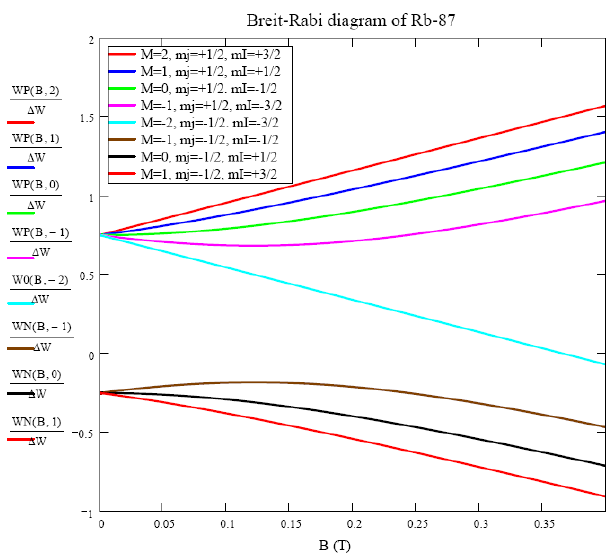
\includegraphics[width=\linewidth]{pictures/breit-rabi.png}
\caption{\textit{Breit-Rabi diagram of $Rb^{87}$ in a magnetic field \cite{ref:3}.}}
\label{fig:7}
\end{minipage}
\end{figure*}
Where, W is the interaction energy and $\Delta$W is the hyperfine splitting 
energy.
\\
Figure \ref{fig:7} shows a plot of the Breit-Rabi equation. The three Zeeman 
levels for the magnetic field are as follows. Weak field is at an x value close 
to zero where the energy splitting varies linearly and the hyperfine 
interaction dominates where the Zeeman effect is the pertubation. The strong 
field region, also known as the Paschen-Back region is x values greater than 2 
where the energy levels are linear once again and depends on the Zeeman effect 
where the hyperfine splitting is taken as the pertubation. The final region 
is the intermediate field region at values greater than zero but less than 2. 
In this region both the hyperfine splitting and the Zeeman effect contribute 
equally to the energy splitting of the electronic orbitals \cite{ref:4}.
\\
In this experiment we are only concerned with the weak field Zeeman effect.

\subsection{Photon absorption in an alkali atom}
\begin{figure*}
\begin{minipage}[t]{\textwidth}
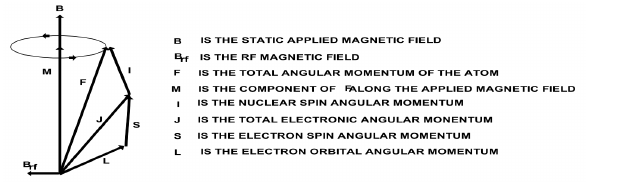
\includegraphics[width=\linewidth]{pictures/all-vectors.png}
\caption{\textit{Magnetic fields and angular momenta involved in the experiment 
\cite{ref:3}.}}
\label{fig:8}
\end{minipage}
\end{figure*}
The lowest electronic state along with the first two excited states of the 
valence electron for a rubidium atom are the following: $^2S_{1/2}$, 
$^2P_{1/2}$ and $^2P_{3/2}$. Where, we will mainly deal with the ground state 
and the first excited state for simplicity.
\\
The transitions from the ground state to the excited state are governed by 
selection rules that are as follows: $\Delta$L = 0,$\pm$1, $\Delta$S = 0 and 
$\Delta$J = 0,$\pm$1. However, the value of L cannot go from 0 to 0 
\cite{ref:3}.
\\
For this experiment we are interested in the amount of light that is absorbed 
or transmitted by the rubidium atoms in a given volume. For this purpose it can 
be useful to use the concept of a cross section of the atoms. In the limit of 
low density this can be represented as.
\begin{equation}
n = n_0e^{-\sigma\rho l}
\label{eqn:15}
\cite{ref:3}
\end{equation}
Where, n and n$_0$ are the incoming and outgoing flux of electrons and $\rho$ 
is the density of the gas.
\\
A similar concept can be employed when talking about a flux of photons.
\begin{equation}
I = I_0 e^{-\sigma_0\rho l}
\label{eqn:16}
\cite{ref:3}
\end{equation}
Where the cross section in this equation is actually the cross section at the 
resonance condition which is much lower than the expected value.
\\
Now we must append to our selection rules for transitions to account for the 
selection rules for the hyperfine splitting which will add that $\Delta$F = 
0,$\pm$1. Additional splitting caused by the magnetic field adds that $\Delta$M 
= 0,$\pm$1.
\\
The selection rule for M can be somewhat different, because since angular 
momentum must always be conserved the photons that are absorbed  must be circularly 
polarized. Of course, if light is circularly polarized we will be adding to 
the angular momentum. The question then becomes how does it change depending on 
the polarization.
\\
It has already been established that only circularly polarized will change the 
angular momentum of the atom. So, depending on the polarization we will get 
addition or subtraction to the angular momentum. That is to say that we will 
have either a +1 or a -1 to the angular momentum, never both.
\\
The lifetime of the transitions will be determined by collision processes. 
It is mentioned that the rubidium glass bulb is filled with a buffer gas that 
is there to decrease the collisions of the atoms with the walls of the 
container and lose its angular momentum. The neon gas dissaallows this from 
happening and since it is a very symmetric atom it will not contribute much to 
the decrease of the angular momentum of the atom \cite{ref:1}.

\subsection{Optical pumping in rubidium}
\begin{figure*}
\begin{minipage}[t]{\textwidth}
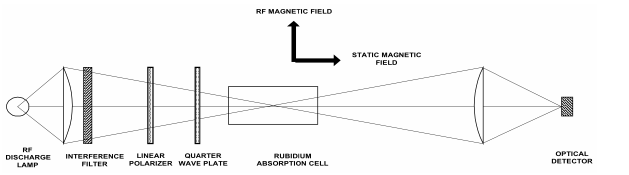
\includegraphics[width=\linewidth]{pictures/rough-apparatus.png}
\caption{\textit{Magnetic fields and angular momenta involved in the experiment
\cite{ref:3}.}}
\label{fig:9}
\end{minipage}
\vfill
\begin{minipage}[t]{\textwidth}
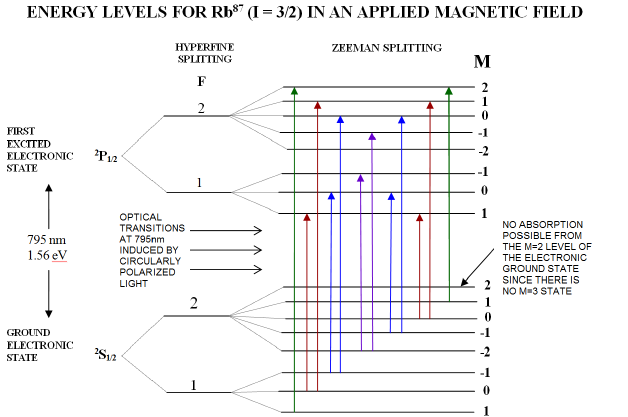
\includegraphics[width=\linewidth]{pictures/energy-lev-trans.png}
\caption{\textit{Transitions involved in the optical pumping of $Rb^{87}$ 
\cite{ref:3}.}}
\label{fig:10}
\end{minipage}
\end{figure*}
In optical pumping we are trying to create a net population 
difference in one state relative to another. From statistical mechanics we know 
that electronic states can settle into a thermal equilibrium where there is no 
net population difference on one state. By making use of the hyperfine 
splitting and the Zeeman effect along with some clever applications of the 
incoming photons we can achieve this.
\\
On figure \ref{fig:10} we see the 
types of transitions that are possible. On the left side of the figure we see 
that there is a large separation between the energy levels that corresponds to 
a transition energy of a 795 nm photon. Then there are smaller gaps that come 
from the hyperfine splitting and then the Zeeman levels.
\\
In order to create this 795 nm photon an RF discharge lamp is used to create 
circulary polarized light at that wavelength. The RF discharge lamp along with 
a general schematic of the experiment is shown on figure \ref{fig:9}. Inside 
the RF discharge there is some $Rb^{87}$ gas along with some metal. When a 
current is passed through the gas it induces a transition to populate the 
first two excited states. By spontaneous emission it then emits two photons, 
one at 795 nm and one at 780 nm. We are only interested in the 795 nm line 
and can filter the 780 nm line by the interference filter \cite{ref:3}.
\\
There is also a linear polarizer that serves a very important purpose. 
Previously it was shown that the M levels can be increased by using circularly 
polarized light. Meaning, we are not interested in the effects of the linearly 
polarized light on the transitions. Why is it important that we do this you 
may ask. The reason is because the $^2P_{1/2}$ state has the highest angular 
momentum when it has a value of M = 2. There is no M = 3 state meaning that once 
the electrons make the transition to the M = 2 state they will accumulate on 
that level until they can relax back to their ground configuration. By this 
method we create a population difference.
\\
One should always be note that the Zeeman effect causes transitions within the 
atomic orbitals where the circularly polarized light causes the transitions 
beween the different energy levels. Should also mention that this is not 
restricted to the positive values since it depends on the polarization 
direction of the light.

\subsection{Zero field transition}
\begin{figure*}
\begin{minipage}[t]{0.44\textwidth}
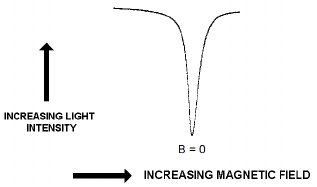
\includegraphics[width=\linewidth]{pictures/zero-field-trans.png}
\caption{\textit{Zero field transition with no RF field \cite{ref:3}.}}
\label{fig:11}
\end{minipage}
\hfill
\begin{minipage}[t]{0.44\textwidth}
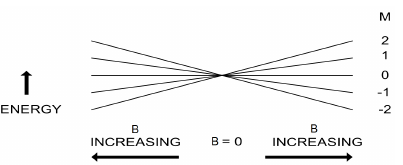
\includegraphics[width=\linewidth]{pictures/energy-zero.png}
\caption{\textit{Energy levels near zero field with no RF field \cite{ref:3}.}}
\label{fig:12}
\end{minipage}
\end{figure*}
Before going further to talk about RF induced transitions we should mention the 
transitions that occur at values of zero magnetic field. The fundamental reason 
this happens is because the atoms are still being irradiated with the photnos 
at the energy to excite the electrons. When the magnetic field is zero there 
are no effects from the hyperfine splitting or the Zeeman effect so there is, 
ideally, only two energy levels and have a completely degenerate system. Where, 
it becomes simple to populate one of them.
This results in the lineshape that is shown on figure \ref{fig:11}.
\\
This can be used to tune the magnetic field of the appartus and cancel off most 
if not all of the outside sources of magnetic fields. The equipment is 
extremely sensitive to tiny changes in magnetic field where a laptop being on 
or off can make a difference in the accuracy of the data.
\\
One of the most prominent sources of outside magnetic field is the field that 
is produced by the Earth and must be cancelled by using a combination of the 
vertical, horizontal coils and lateral positioning of the apparatus.

\subsection{Transient effects}
Throughout this report we have been considering the optical pumping to happen 
only when the RF has been constantly on. Now we will consider the case when the 
RF signal is turned off and on at a certain frequency.
\\
When we are at resonance the Larmor frequency for the weak field Zeeman effect 
is given by.
\begin{equation}
\begin{aligned}
\omega_0 &= 2\pi\nu_0 
         &= g_F\frac{\mu_B}{\hbar}B_0
\label{eqn:17}
\cite{ref:3}
\end{aligned}
\end{equation}
Where, $\nu_0$ is given by equation \ref{eqn:11} and $g_F$ by equation 
\ref{eqn:10}. We can then define the gyromagnetic ratio, $\gamma$, as.
\begin{equation}
\gamma = g_F\frac{\mu_B}{\hbar}
\label{eqn:18}
\cite{ref:3}
\end{equation}
We can then write the Larmor frequency as.
\begin{equation}
\omega_0 = \gamma B_0
\label{eqn:19}
\cite{ref:3}
\end{equation}
The equations above are very similar to those employed in Nuclear Magnetic 
Resonance.
\center
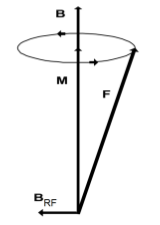
\includegraphics[width=0.4\linewidth]{pictures/rf-larmor.png}
\captionof{figure}{\textit{F vector an the precession about the magnetic field 
with perpendicular field $B_{RF}$ \cite{ref:3}.}}
\label{fig:13}
\justify
Figure \ref{fig:13} shows how the total atomic angular momentum precesses 
about the magnetic field, $B$, when a perpendicular field tuned to the Larmor 
frequency, $B_RF$.

\section{Experimental Set-Up}
For this experiment we are using a TeachSpin set-up that provides us access to 
the equipment that is necessary to be able to carry out the experiment without 
much dificulty or needing to set-up very complicated equipment.
\subsection{Rubidium Discharge Lamp}
The rubidium discharge lamp consists of an RF oscilator, oven and gas bulb. In 
the bulb there is a mixture of gas containing rubidium gas and a buffer gas. 
The buffer gas in the bulb is xenon. The remaining gas is a mixture of 
$Rb^{85}$ and $Rb^{87}$ with concentrations of about 36\% and 64\% respectively.
The oven is set to a temperature of 115$^0$ C.
\\
The lamp takes 10 to 20 minutes in order to fully turn on and be able to 
equalize the temperature inside the gas bulb. It should be noted that the 
rubidium atoms emmit light at the 795 nm range which is in the near infrared. 
One may be able to see some light coming from the lamp, but this light may be 
due to the xenon spectral line or higher lines of rubidium \cite{ref:3}.
\\
We are only interested in the 795 nm range line.

\subsection{Detector}
\begin{figure*}
\begin{minipage}[t]{\textwidth}
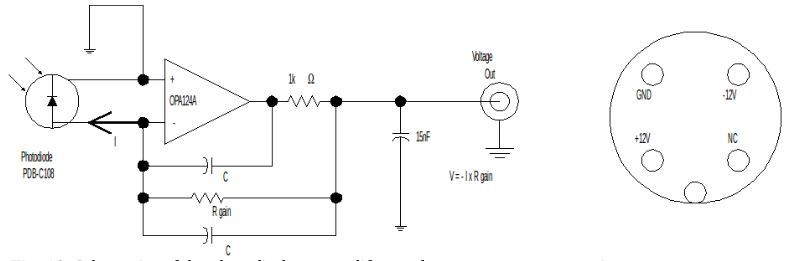
\includegraphics[width=\linewidth]{pictures/detector-schem.png}
\caption{\textit{General Schematic of the photodiode detector with preamplifier 
and preamp power connections \cite{ref:3}.}}
\label{fig:14}
\end{minipage}
\end{figure*}
The detector is a PDB-C108 silicon photodiode from Photonic Detectors Inc. 
\cite{ref:3} With an active area of 0.25 inches in diameter and a spectral 
response in the 795 nm range of 0.6 A/W. Figure \ref{fig:14} gives a general 
schematic of the photodiode with some of the connections. The preamp is a 
current-to-voltage converter with three gain settings selectable by a switch 
on the detector itself.
\\
The photodiode preamplifier has a voltage range of 0.0 V to 11.5 V and it 
should be kept in mind to avoid saturating the signal.
\begin{minipage}[t]{\linewidth}
\center
\begin{tabular}{|c|c|c|}
\hline
Gain Resistor & Low pass 3dB point & Noise \\ 
(M$\Omega$) $\pm$ 5\% & (kHz) $\pm$ 10\% & ($\mu V_{pp}$) \\ \hline
1 & 12.0 & 20 \\ \hline
3 & 8.0 & 40 \\ \hline
10 & 5.0 & 100 \\ \hline
\end{tabular}
\captionof{table}{\textit{Photodiode preamplifier specifications \cite{ref:3}.}}
\label{tbl:1}
\end{minipage}
The signal from the preamp is on a coaxial BNC connector labeled Detector that 
feeds into the main housing for the analysis. This can be used to connect 
the cable directly to an osciloscope and see what is being read.
\\
The electronics houses the following sections that can help to adjust the 
signal from the detector \cite{ref:3}.
\begin{enumerate}[label=\alph*).]
\item DC offset: 0-10 V DC Set by a ten turn potentiiometer and fine control 
adjustment 0-20 mV set by a one turn potentiometer. At low gain settings the 
fine adjustment knob will not be very useful due to the scaling difference.
\item Gain: 1,2,5 ... 100 Adjustable gain knob that will increase the signal 
gain. The maximum value is 1000.
\item Low Pass filter: A two pole low pass filter with time constants: min., 
1 ms, 10 ms, 100 ms, 1 s, 3s. When the min. value is selected, the frequency 
response is determined by the gain setting of the preamplifier.
\item Meter: Displays the voltage reading from the detector output. The range 
is from -4 to +4 V with a multiplier toggle switch to increase to a range of 
-8 to +8 V.
\end{enumerate}

\subsection{Optics}
\begin{figure*}
\begin{minipage}[t]{\textwidth}
\center
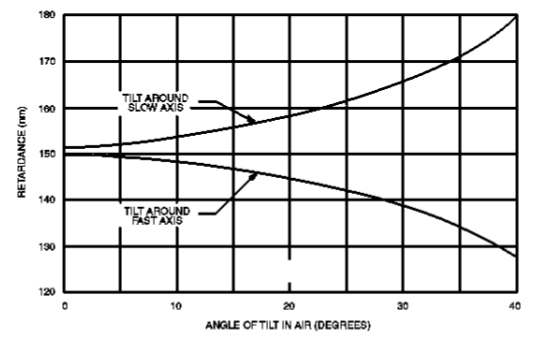
\includegraphics[width=0.6\linewidth]{pictures/quarter-wave.png}
\caption{\textit{Tilt tuning of the quarter wavelength plate \cite{ref:3}.}}
\label{fig:15}
\end{minipage}
\end{figure*}
In this section we will go into the optics that are used for this experiment. 
The optics that will be discussed are: plano-convex lenses, 
interference filter, polarizers, quarter wavelength plate.
\begin{enumerate}[label=\alph*).]
\item Two plano-convex lenses: Diameter 50 mm, focal length 50 mm.
\item Interference filter: Diameter 50 mm. This filter is chosen since it has 
the ability to absorb the 780 nm line that is emmited and still transmit the 
795 nm line that is of interest in the experiment.
\item Two linear polarizers on rotable mounts: Diameter 50 mm. The linear 
polarizer will be used to filter out other polarizations of light so that they 
can be converted into circularly polarized light with the help of a quarter 
wavelength plate.
\item Quarter wavelength plate on rotable mount: Diameter 50 mm, "optical 
thickness" 205 $\pm$ 5 nm. When properly oriented, the plate can convert 
linearly polarized light into circularly polarized light. The plate has 
different optical axes which have different indices of refraction that will 
slow down the light beam. To produce circularly polarized light, place the 
quarter wave plate at a 45$^0$ angle to the linear polarizer.
\\
Figure \ref{fig:15} gives the retardation about the different axial tilt. 
Tuning the optical thickness (retardation) can be accomplished by rotating the 
plates.
\item Alignment: Throughout the experiment the optics may need to be aligned to 
be able to get the best results from the equipment. One way to do this is to 
maximize the signal gotten from the detector by moving the lenses until the 
signal reaches a maximum value. In theory this should work since the light 
incident to the lenses should be made to be linearly aligned and then re-focus 
into the detector to get the signal reading. If we do not get a maximum value 
there are two thing that can be happening. The light that is coming from the 
lamp is not being spread into a parallel beam correctly or the light that is 
going into the detector is not being refocused properly.
\\
We shall look at the first problem. One possible way to troubleshoot the 
problem is to use a sheet of whitepaper and place it infront of the lens. 
Remember that the light that we are able to see with the slight purple color 
is the light that may be due to transitions in the xenon gas or higher energy 
excitations in the rubidium atoms. So, we cannot do this after the interference 
filter as we will not be able to see the light beam nor properly adjust the 
lens position. By moving the paper back and forth one should be able to see 
that the beam of light does not change in size which we will see as a circle. 
If it does diverge slightly change the lens position until it does not 
diverge anymore and the circle is at its maximum diameter.
\\
Now we shall look at the second problem which will be at the detector. For this 
we can place the quarter wave plate and the linear polarizer infront of the 
discahrge lamp. Due 
to the fact that the emtire aparatus is bolted onto the rail and table we will 
not be able to use the same troubleshooting method as we did before, since we 
cannot see the light beam. What we 
must do is to read a signal either on the osciloscope or a voltmeter and 
maximize the signal. To do this change the position of the lens on the rail and assuming that the first lens was set to its correct position the second should 
be in the correct position when the signal from the detector is at a maximum. 
This is because, the light beam that incident on the lens is supposedly 
parralel and constant so the lens should refosus the light back into a single 
point and this point should be at the detector.
\\
It is important to check the heigth of the optics which should be set to a 
heigth of approximately 3.5 inches.
\end{enumerate}

\subsection{Temperature regulation}
The following component make up the cell temperature regulation system 
\cite{ref:3}.
\begin{enumerate}[label=\alph*).]
\item Temperature regulator: Proportional, Integral, Derivative (PID) 
temperature controller with associated electronics. The settings for the PID 
are preset in the electronics box and cannot be change without changing the 
inner electronics.
\item Temperature probe: Type T (Copper - Constantan) Thermocouple (5 $\mu$m 
wire). Constantan is magnetic, however, the wire was chosen to be so small so 
that the effect of its magnetic field on the magnetic field in the sample can 
be neglected.
\item Oven: The oven consists of the following components.
\begin{enumerate}[label=\arabic*).]
\item Rubidium cell: Glass bulb that contains the rubidium sample that is to be 
studied in the experiment.
\item Cell holder: A foam insert that holds the sample.
\item Heater: The heater is an open-ended glass heater that is wrapped with 
non-magnetic bifilar wound heater wire. The resistance is measured to be 50 
$\Omega$.
\item Insulation: Foam layer surrounding the heater.
\item Oven casing: A Plexiglass cylinder. Has endcaps of 50 mm optical windows. 
Holes in the casing allow wires to be run into the oven.
\end{enumerate}
\item Operation: On the front face of the electronics box there is a controller 
window with three buttons that control the menu up and down respectively. To 
set a temperature one must press the menu button and cycle to SP (Set Point) 
and using the up and down buttons one can set the desired temperature in 
centigrade. To view the current temperature one can press the menu button again 
and press it again to show the PRoC on the display. By leaving it on this 
setting it will display the measured temperature.
\\
Do note that setting the temperature takes a very long time (20-30 minutes). 
So, the first thing that should be done when starting the lab should be to set 
the temperature and allow it to settle.
\\
The minimum temperature is ambient room temperature where the max is 
approximately 100$^0$ C.
\end{enumerate}

\subsection{Magnetic Fields}
All the DC magnetic fields are produced by magnetic coils that are placed in a 
Helmholtz configuration. There are three magnetic coils whose specs are known.
\begin{minipage}[t]{\linewidth}
\center
\begin{tabular}{|c|c|c|}
\hline
{} & Mean Radius & Turns/Side \\ {} & (cm) & {} \\ \hline
Vertical Field & 11.735 & 20 \\ \hline
Horizontal Field & 15.79 & 154 \\ \hline
Sweep field & 16.39 & 11 \\ \hline
\end{tabular}
\captionof{table}{\textit{Mean Radius and turns given values for the coils 
\cite{ref:3}.}}
\label{tbl:2}
\begin{tabular}{|c|c|c|}
\hline
{} & Field/Amp & Max Field \\ 
{} & ($T\times10^{-4}/A$) & ($T\times10^{-4}$) \\ \hline
Vertical Field & 1.5 & 1.5 \\ \hline
Horizontal Field & 8.8 & 22.0 \\ \hline
Sweep field & 0.60 & 0.60 \\ \hline
\end{tabular}
\captionof{table}{\textit{Field/Amp and Maximum field specs for the coils. The 
Field/Amp specs are approximate \cite{ref:3}.}}
\label{tbl:3}
\end{minipage}

\section{Results and Discussion}
\subsection{Absorption of $Rb$ resonance radiation by atomic $Rb$}
\begin{figure*}
\begin{minipage}[t]{\textwidth}
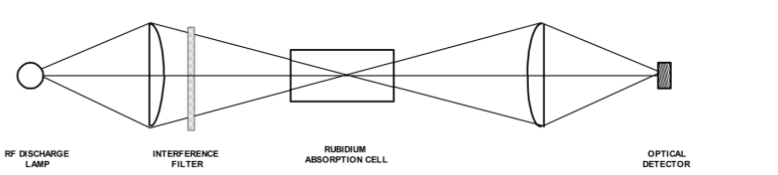
\includegraphics[width=\linewidth]{pictures/i-schem.png}
\caption{\textit{General schematic of the set-up for part i \cite{ref:3}.}}
\label{fig:16}
\end{minipage}
\begin{minipage}[t]{0.45\textwidth}
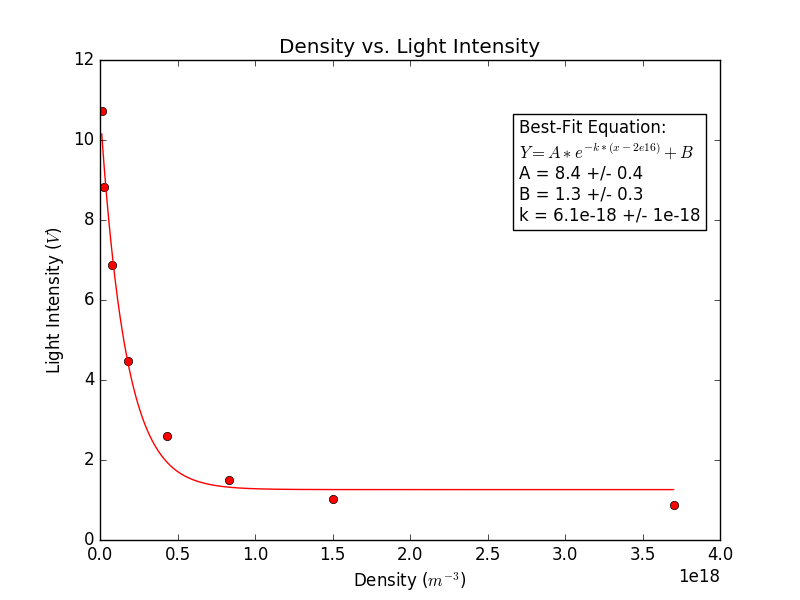
\includegraphics[width=\linewidth]{pictures/density-light.png}
\caption{\textit{Light intensity as a function of density of rubidium atoms at 
given temperature values.}}
\label{fig:17}
\end{minipage}
\hfill
\begin{minipage}[t]{0.45\textwidth}
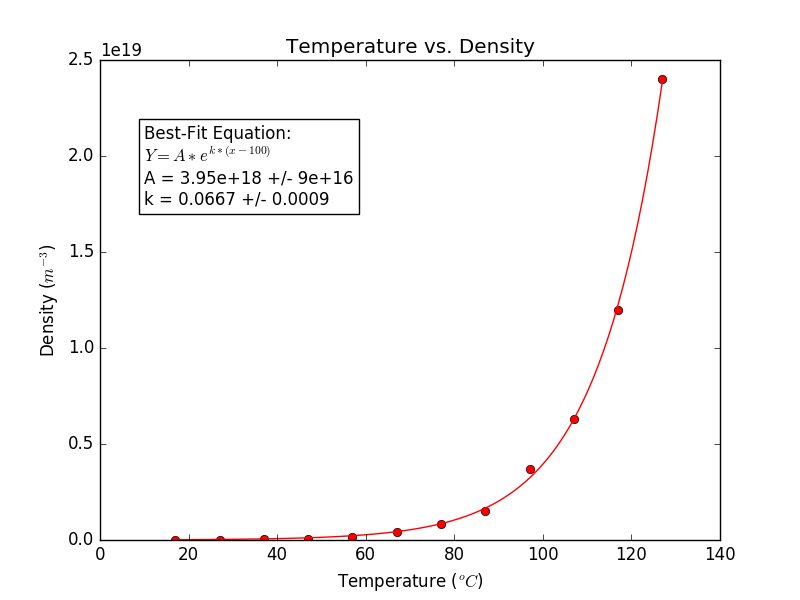
\includegraphics[width=\linewidth]{pictures/temp-density.png}
\caption{\textit{Density of rubidium atoms as a function of temperature.}}
\label{fig:18}
\end{minipage}
\end{figure*}
For this part of the experiment we are trying to make an approximate 
measurement of the cross sectional area of atomic rubidium. The method we used 
to do so was by irradiating the sample with photons and measuring the 
intensity of the light as a function of temperature. A general schematic is 
outlined on figure \ref{fig:16}. The schematic shows us that we should only 
have the two convex-plano lenses and the interference filter to make the 
measurements.
\\
The data that was taken is given in the following table.
\begin{minipage}{\linewidth}
\center
\begin{tabular}{|c|c|}
\hline
Temperature (\textsuperscript{0}C) & Intensity (V) \\ \hline
27.0 & 10.727 \\ \hline
37.0 & 8.819 \\ \hline
47.0 & 6.875 \\ \hline
57.0 & 4.473 \\ \hline
67.0 & 2.602 \\ \hline
77.0 & 1.496 \\ \hline
87.0 & 1.035 \\ \hline
97.0 & 0.866 \\ \hline
\end{tabular}
\captionof{table}{\textit{Data taken for part i of the experiment.}}
\label{tbl:4}
\end{minipage}
We then fitted the data with an exponential curve that would follow the 
form of equation \ref{eqn:16}, except with an added error term. The equation 
that was fitted using Python was.
\begin{equation}
Y = Ae^{-k(x-2e16)}+B
\label{eqn:20}
\end{equation}
Where, k is given as the product of the cross sectional area times the path 
length, x is the density of the rubidium atoms which was given in the 
following table and y are the measured intensity values from the data.
\begin{minipage}{\linewidth}
\center
\begin{tabular}{|c|c|}
\hline
Temperature & Density \\ 
($^0C$) & ($m^{-3}$) \\ \hline
17 & $3.3\times10^{15}$ \\ \hline
27 & $1.1\times10^{16}$ \\ \hline
37 & $2.9\times10^{16}$ \\ \hline
47 & $7.5\times10^{17}$ \\ \hline
57 & $1.8\times10^{17}$ \\ \hline
67 & $4.3\times10^{17}$ \\ \hline
77 & $8.3\times10^{17}$ \\ \hline
87 & $1.5\times10^{18}$ \\ \hline
97 & $3.7\times10^{18}$ \\ \hline
107 & $6.3\times10^{18}$ \\ \hline
117 & $1.2\times10^{19}$ \\ \hline
127 & $2.4\times10^{19}$ \\ \hline
\end{tabular}
\captionof{table}{\textit{Density of rubidium atoms as a function of 
temperature \cite{ref:3}.}}
\label{tbl:5}
\end{minipage}
Using all of the values and the curve fitting functions in Python the cross 
sectional area was found to be: $1.8\times10^{-16}$ $\pm$ $0.3\times10^{-16}$ 
m\textsuperscript{2}. The data was plotted on figure \ref{fig:17}.
\\
We also plotted the data that is given on table \ref{tbl:5} and fitted an 
exponential curve to the data using Python. The results are shown on figure 
\ref{fig:18}.
\\
A quick note on the fitting functions. The values that are subtracting from x 
were chosen to be those because we needed to shift the entire curve and they 
gave the lowest uncertainty values comparatively. The B term in equation 
\ref{eqn:20} is an error term that accounts for outside sources of light that 
are not eliminated by the aparatus.

\subsection{Low field resonances}
\begin{figure*}
\center
\begin{minipage}[t]{\textwidth}
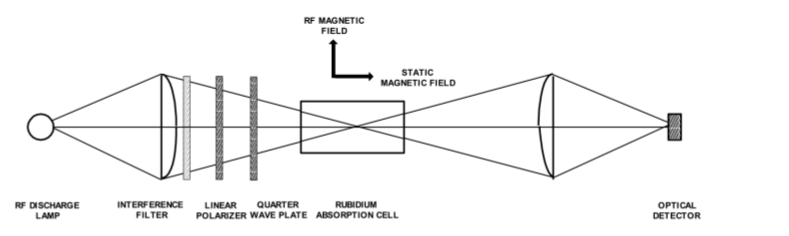
\includegraphics[width=\linewidth]{pictures/ii-schem.png}
\caption{\textit{General schematic for part ii of the experiment \cite{ref:3}.}}
\label{fig:19}
\end{minipage}
\begin{minipage}[t]{0.45\textwidth}
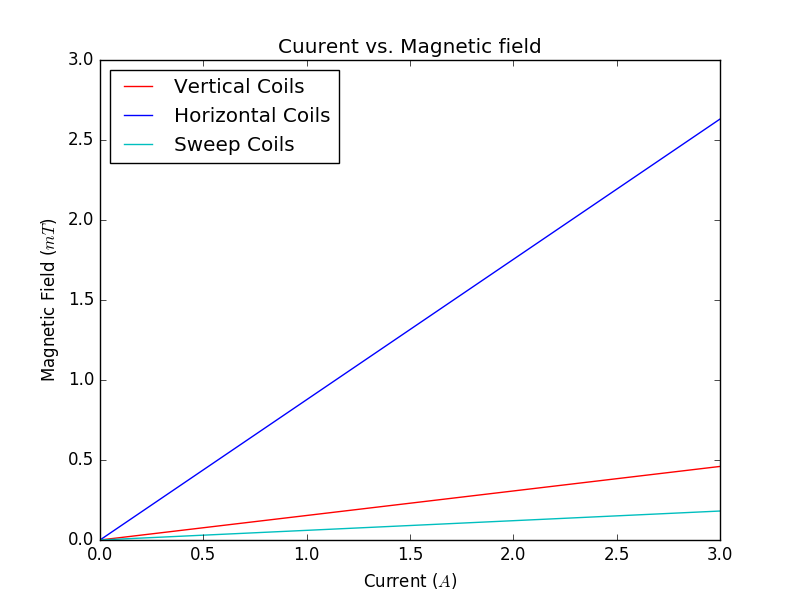
\includegraphics[width=\linewidth]{pictures/current-field.png}
\caption{\textit{Magnetic field as a function of current for the three magnetic 
coils.}}
\label{fig:20}
\end{minipage}
\hfill
\begin{minipage}[t]{0.45\textwidth}
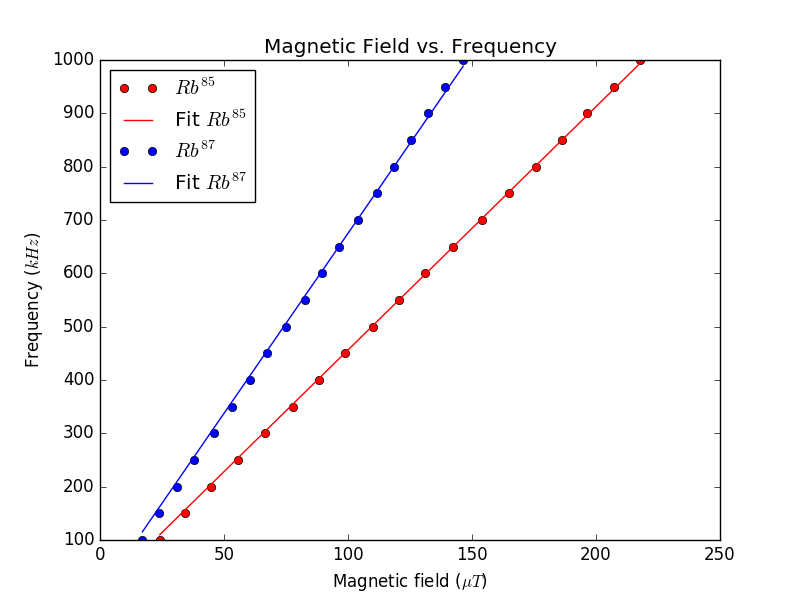
\includegraphics[width=\linewidth]{pictures/field-frequency.png}
\caption{\textit{Frequency as a function of magnetic field.}}
\label{fig:21}
\end{minipage}
\end{figure*}
For this part of the experiment we began using the magnetic fields to be able 
to create the weak field Zeeman effect and hyperfine splitting. The general 
set-up for this part is given on figure \ref{fig:19}. We then found the 
magnetic fields as a function of current using the equation.
\begin{equation}
B = \frac{8\mu_0 NI}{R\sqrt{125}}
\label{eqn:21}
\cite{ref:3}
\end{equation}
Where, $\mu_0$ is the permeability constant, N and R are the turns and mean 
radius values that are given in table \ref{tbl:2} and \ref{tbl:3} and I was 
varied. During the experiment we measure the voltage value that is running 
through the coils but on the electrical box we can see the resistances that 
are given for each of the coils and by Ohm's law can calculate the current.
\subsubsection{Zero field transition:}
In the theory section we talked about the zero field transition and for the 
experiment we had to find this transition so as to be able to calibrate our 
maesured magnetic field values so that there was no outside field 
interferences. A screenshot was taken of the zero field transition.
\center
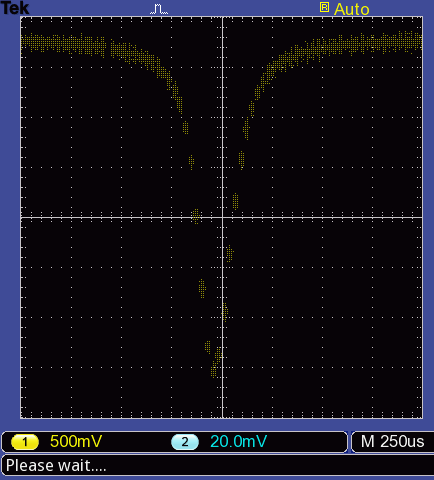
\includegraphics[width=\linewidth]{pictures/zero-field-data.png}
\captionof{figure}{\textit{Zero field transition taken during part ii of the 
experiment in XY mode of the oscilloscope.\\}}
\label{fig:22}
\justify
What we found was that the zero field transition had to be found by changing 
both the fields in the horizontal and vertical components. The vertical field 
was found to be 51.2 $\pm$ 0.3 $\mu$T. The horizontal was found to be 10.1 
$\pm$ 0.1 $\mu$T when assuming the error in the voltmeter readings to be 
0.002 V. We set the temperature to be $50^oC$.

\subsubsection{Measurement of $g_F$ factors and nuclear spins:}
In this section we wanted to find the $g_F$ factors that we defined in equation 
\ref{eqn:10} along with the nuclear spin (I). The method that we used to do 
this was by using an RF signal we varied the signal from 100 kHz up to 1 GHz in 
intervals of 50 kHz and measured the voltage on the coils at the moment that 
the rubidium atoms underwent the transition. The first transition at the 
resonance condition was taken as a screenshot from the oscilloscope and shown 
below.
\center
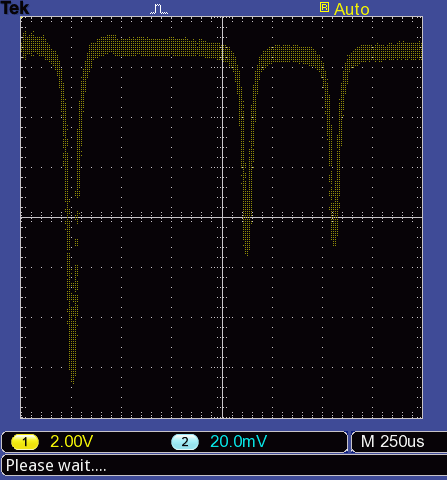
\includegraphics[width=\linewidth]{pictures/low-field-resonance.png}
\captionof{figure}{\textit{Screenshot of the first resonance condition at low 
fields at a frequency value of 100 kHz.}}
\label{fig:23}
\justify
Data was taken at each frequency value and the values of the sweep field and 
horizontal field voltages, current and magnetic field were calculated along 
with the total field value. The data is shown on the table on the next page.

\twocolumn[
\begin{@twocolumnfalse}
\center
\begin{tabular}{|c|c|c|c|c|c|c|c|c|}
\hline
\multicolumn{9}{c}{Rb\textsuperscript{85}} \\ \hline
{} & \multicolumn{3}{c}{Sweep field coil} &
\multicolumn{3}{c}{Horizontal field coil} && Combined \\ \hline
Frequency & Voltage & Current & Field & Voltage & Current & Field && Field \\  
(kHz) & (V) & (A) & ($\mu T$) & (V) & (A) & ($\mu T$) && ($\mu T$) \\ \hline
100.0 & 0.5134 & 0.5134 & 30.9824 & 0.00184 & 0.0037 & 3.2272 && 24.0712 \\ \hline
150.0 & 0.685 & 0.685 & 41.338 & 0.00184 & 0.0037 & 3.2272 && 34.4268 \\ \hline
200.0 & 0.8575 & 0.8575 & 51.7479 & 0.00184 & 0.0037 & 3.2272 && 44.8368 \\ \hline
250.0 & 0.7743 & 0.7743 & 46.727 & 0.0108 & 0.0216 & 18.9425 && 55.5311 \\ \hline
300.0 & 0.579 & 0.579 & 34.9411 & 0.0239 & 0.0478 & 41.919 && 66.7218 \\ \hline
350.0 & 0.5596 & 0.5596 & 33.7704 & 0.0308 & 0.0616 & 54.0212 && 77.6532 \\ \hline
400.0 & 0.7333 & 0.7333 & 44.2527 & 0.0308 & 0.0616 & 54.0212 && 88.1356 \\ \hline
450.0 & 0.9069 & 0.9069 & 54.7291 & 0.0308 & 0.0616 & 54.0212 && 98.6119 \\ \hline
500.0 & 0.7126 & 0.7126 & 43.0036 & 0.044 & 0.088 & 77.1731 && 110.0383 \\ \hline
550.0 & 0.7828 & 0.7828 & 47.2399 & 0.0477 & 0.0954 & 83.6627 && 120.7643 \\ \hline
600.0 & 0.933 & 0.933 & 56.3041 & 0.0485 & 0.097 & 85.0658 && 131.2316 \\ \hline
650.0 & 0.7178 & 0.7178 & 43.3174 & 0.0623 & 0.1246 & 109.2701 && 142.4491 \\ \hline
700.0 & 0.4578 & 0.4578 & 27.627 & 0.0778 & 0.1556 & 136.4561 && 153.9448 \\ \hline
750.0 & 0.446 & 0.446 & 26.9149 & 0.0844 & 0.1688 & 148.0321 && 164.8087 \\ \hline
800.0 & 0.4736 & 0.4736 & 28.5805 & 0.0897 & 0.1794 & 157.3279 && 175.7701 \\ \hline
850.0 & 0.6453 & 0.6453 & 38.9422 & 0.0897 & 0.1794 & 157.3279 && 186.1318 \\ \hline
900.0 & 0.8175 & 0.8175 & 49.334 & 0.0897 & 0.1794 & 157.3279 && 196.5236 \\ \hline
950.0 & 0.8299 & 0.8299 & 50.0823 & 0.0954 & 0.1908 & 167.3254 && 207.2693 \\ \hline
1000.0 & 0.9125 & 0.9125 & 55.067 & 0.0986 & 0.1972 & 172.938 && 217.8666 \\ \hline
\end{tabular}
\captionof{table}{\textit{Data taken and calculated from known values. The 
Voltage columns and the frequency columns are from data that was taken.\\}}
\label{tbl:6}
\begin{tabular}{|c|c|c|c|c|c|c|c|c|}
\hline
\multicolumn{9}{c}{Rb\textsuperscript{87}} \\ \hline
{} & \multicolumn{3}{c}{Sweep field coil} & 
\multicolumn{3}{c}{Horizontal field coil} && Combined \\ \hline
Frequency & Voltage & Current & Field & Voltage & Current & Field && Field \\ 
(kHz) & (V) & (A) & ($\mu T$) & (V) & (A) & ($\mu T$) && ($\mu T$) \\ \hline
100.0 & 0.3974 & 0.3974 & 23.9821 & 0.00184 & 0.0037 & 3.2272 && 17.0709 \\ \hline
150.0 & 0.511 & 0.511 & 30.8375 & 0.00184 & 0.0037 & 3.2272 && 23.9264 \\ \hline
200.0 & 0.6265 & 0.6265 & 37.8076 & 0.00184 & 0.0037 & 3.2272 && 30.8965 \\ \hline
250.0 & 0.4843 & 0.4843 & 29.2262 & 0.0108 & 0.0216 & 18.9425 && 38.0304 \\ \hline
300.0 & 0.2327 & 0.2327 & 14.0428 & 0.0239 & 0.0478 & 41.919 && 45.8235 \\ \hline
350.0 & 0.1553 & 0.1553 & 9.372 & 0.0308 & 0.0616 & 54.0212 && 53.2548 \\ \hline
400.0 & 0.2728 & 0.2728 & 16.4628 & 0.0308 & 0.0616 & 54.0212 && 60.3456 \\ \hline
450.0 & 0.388 & 0.388 & 23.4148 & 0.0308 & 0.0616 & 54.0212 && 67.2976 \\ \hline
500.0 & 0.1347 & 0.1347 & 8.1288 & 0.044 & 0.088 & 77.1731 && 75.1636 \\ \hline
550.0 & 0.1486 & 0.1486 & 8.9676 & 0.0477 & 0.0954 & 83.6627 && 82.4919 \\ \hline
600.0 & 0.2413 & 0.2413 & 14.5618 & 0.0485 & 0.097 & 85.0658 && 89.4893 \\ \hline
650.0 & 0.3565 & 0.3565 & 21.5138 & 0.0485 & 0.097 & 85.0658 && 96.4413 \\ \hline
700.0 & 0.2671 & 0.2671 & 16.1188 & 0.0558 & 0.1116 & 97.8696 && 103.85 \\ \hline
750.0 & 0.1556 & 0.1556 & 9.3901 & 0.064 & 0.128 & 112.2518 && 111.5035 \\ \hline
800.0 & 0.2695 & 0.2695 & 16.2636 & 0.064 & 0.128 & 112.2518 && 118.3771 \\ \hline
850.0 & 0.2678 & 0.2678 & 16.161 & 0.068 & 0.136 & 119.2676 && 125.2902 \\ \hline
900.0 & 0.384 & 0.384 & 23.1734 & 0.068 & 0.136 & 119.2676 && 132.3026 \\ \hline
950.0 & 0.4989 & 0.4989 & 30.1073 & 0.068 & 0.136 & 119.2676 && 139.2365 \\ \hline
1000.0 & 0.5807 & 0.5807 & 35.0437 & 0.0693 & 0.1386 & 121.5477 && 146.4531 \\ \hline
\end{tabular}
\captionof{table}{\textit{Data taken and calculated from known values. The 
Voltage columns and the frequency columns are from data that was taken.\\}}
\label{tbl:7}
\end{@twocolumnfalse}]
The data from tables \ref{tbl:5} and \ref{tbl:6} is included under the 
frequency and the voltage columns for the the sweep field and the horizontal 
field coil. The currents were calculated from Ohm's law where the sweep field 
had a 1 $\Omega$ resistor and the horizontal field had a 0.5 $\Omega$ resistor. 
The fields were calculated using equation \ref{eqn:21}. The combined field was 
found by adding the magnetic fields from both coils and then subtracting the 
value of the zero field magnetic field value. 
\\
A plot of the frequency as a function of the combined magnetic field is shown 
on figure \ref{fig:21}. Using equation \ref{eqn:11} it is easy to see the 
linear relationship between the slope and the $g_F$ factor which when the 
equation is solved for the value we get values of 0.3260 $\pm$ 0.0005 and 0.482 
$\pm$ 0.001 for $Rb^{85}$ and $Rb^{87}$ respectively. By then having the $g_F$ 
factor we can solve for the nuclear angular momentum (I) by rewriting equation 
\ref{eqn:10} for I and we get the algebraic expression.
\begin{equation}
\begin{aligned}
0 = 2&I^2g_F + 2I\left(g_F+J\left[2g_F-g_J\right]\right)
\\
      &- 2J\left(J+1\right)\left(g_J-g_F\right)
\label{eqn:22}
\end{aligned}
\end{equation}
Where, $g_F$ has just been calculated, $g_J$ is the Lande g-factor, J is equal 
to 1/2. Equation \ref{eqn:22} takes the form of a quadratic and can be solved 
for I and when taking the positive roots the values that are gotten for the 
nuclear spin are 2.571 and 1.576 for $Rb^{85}$ and $Rb^{87}$ respectively.

\subsection{Quadratic Zeeman Effect}
\begin{figure*}
\begin{minipage}[t]{0.45\linewidth}
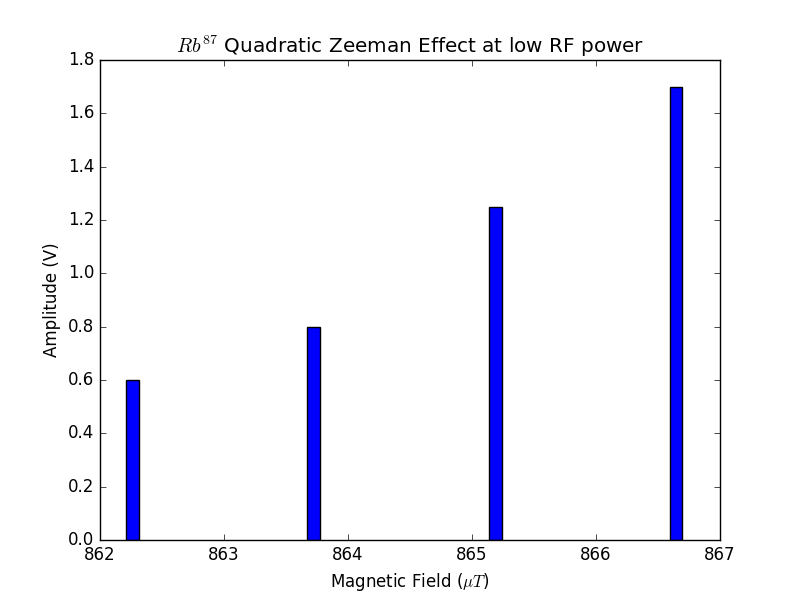
\includegraphics[width=\linewidth]{pictures/rb87-low.png}
\caption{\textit{$Rb^{87}$ quadratic zeeman effect at low RF power}}
\label{fig:24}
\end{minipage}
\hfill
\begin{minipage}[t]{0.45\linewidth}
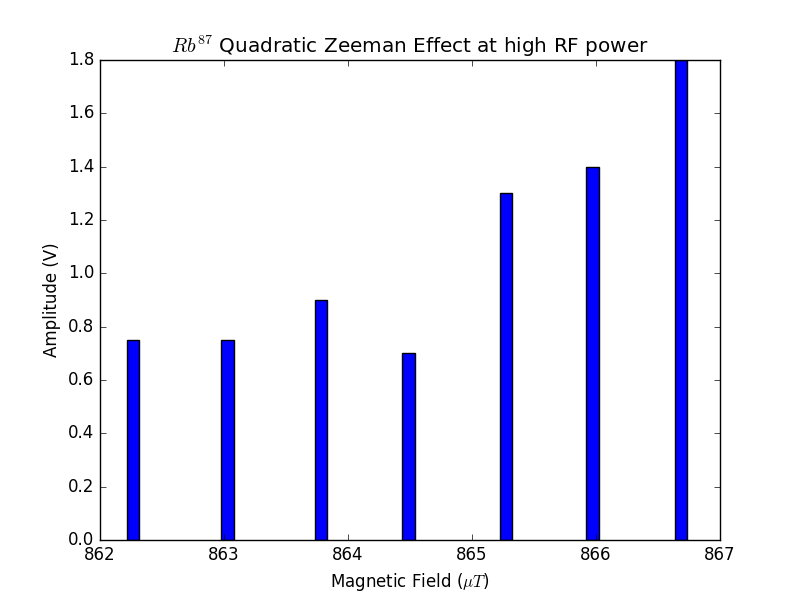
\includegraphics[width=\linewidth]{pictures/rb87-high.png}
\caption{\textit{$Rb^{87}$ double quadratic zeeman effect at high RF power}}
\label{fig:25}
\end{minipage}
\vfill
\begin{minipage}[t]{0.45\linewidth}
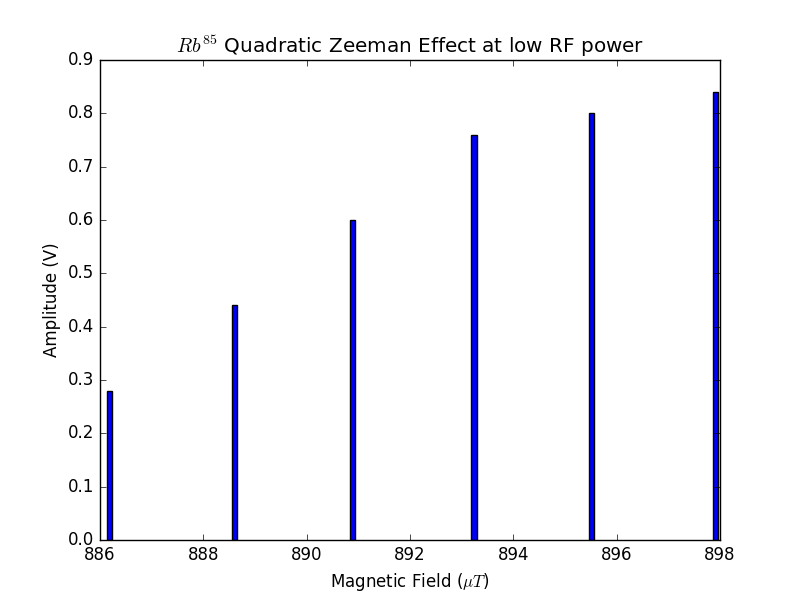
\includegraphics[width=\linewidth]{pictures/rb85-low.png}
\caption{\textit{$Rb^{85}$ quadratic zeeman effect at low RF power}}
\label{fig:26}
\end{minipage}
\hfill
\begin{minipage}[t]{0.45\linewidth}
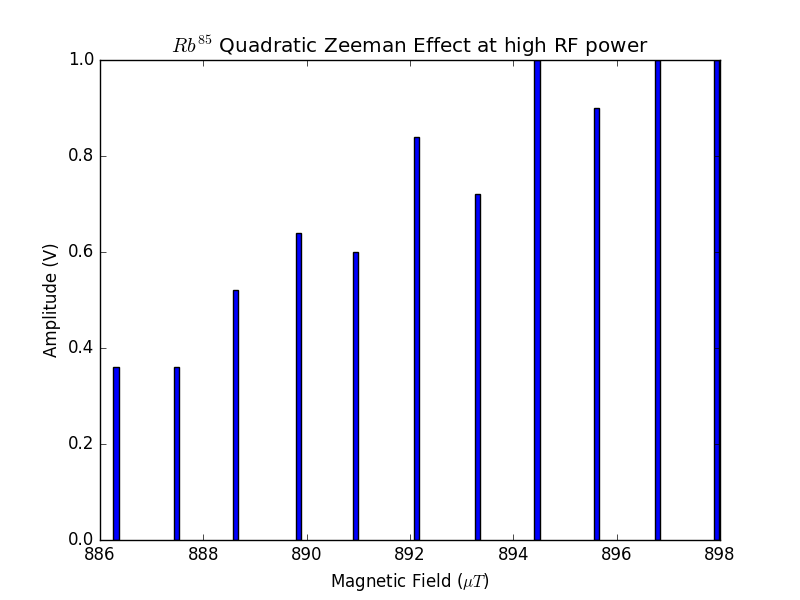
\includegraphics[width=\linewidth]{pictures/rb85-high.png}
\caption{\textit{$Rb^{85}$ double quadratic zeeman effect at high RF power}}
\label{fig:27}
\end{minipage}
\end{figure*}
For this part of the experiment we studied the Zeeman resonances of both 
isotopes. We will study the region in which the energy level splitting is no 
longer linear nor equally spaced and there will be a total of 2F resonances. 
The relative intensities of the signals depend on the pumping conditions.

\subsubsection{$Rb^{87}$ quadratic Zeeman effect}
For this part of the experiment we used the following settings to view the 
quadratic Zeeman effect at low RF power for the $Rb^{87}$.
\\
Detector amplifier gain = 20 \\
Mutiplier = 20 \\
$\nu$ = 5.95 MHz \\
Time constant = 100 ms \\
RF amplifier gain = 3 \\
Sweep time = 50 s \\
Horizontal Field current = 0.9872 A \\
RF amplitude = 1 V \\
\\
The data that was collected is the following.
\begin{minipage}{\linewidth}
\center
\begin{tabular}{|c|c|c|}
\hline
Peak & Amplitude (500 mV) & Voltage (V) \\ \hline
1 & 1.2 & 0.1095 \\ \hline
2 & 1.6 & 0.1337 \\ \hline
3 & 2.5 & 0.1580 \\ \hline
4 & 3.4 & 0.1821 \\ \hline
\end{tabular}
\captionof{table}{\textit{Data taken for low RF power quadratic Zeeman effect \\}}
\label{tbl:8}
\end{minipage}
The plot of the data is shown on figure \ref{fig:24} where the Voltage column 
is the voltage measured for the sweep field coil. To get the magnetic field we 
added the magnetic fields of the sweep and the horizontal magnetic coils and 
subtracted the zero field value.
\\
The screenshot of the data that was taken on the oscilloscope is shown below.
\center
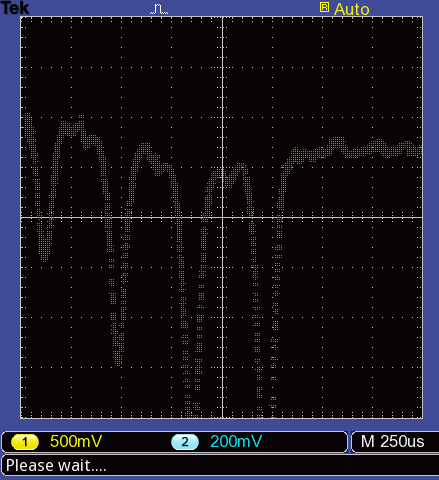
\includegraphics[width=\linewidth]{pictures/rb87-low-raw.png}
\caption{\textit{Quadratic Zeeman effect of $Rb^{87}$ at low RF power \\ }}
\justify
Now we will consider the double quadratic Zeeman effect. For this we used the 
settings.
\\
Detector amplifier gain = 20 \\
Mutiplier = 20 \\
$\nu$ = 5.95 MHz \\
Time constant = 100 ms \\
RF amplifier gain = 3 \\
Sweep time = 50 s \\
Horizontal Field current = 0.9872 A \\
RF amplitude = 2.5 V \\
\\
The data collected was the following.
\begin{minipage}{\linewidth}
\center
\begin{tabular}{|c|c|c|}
\hline
Peak & Amplitude (500 mV) & Voltage (V) \\ \hline
1 & 1.5 & 0.1096 \\ \hline
2 & 1.5 & 0.1222 \\ \hline
3 & 1.8 & 0.1347 \\ \hline
4 & 1.4 & 0.1464 \\ \hline
5 & 2.6 & 0.1594 \\ \hline
6 & 2.8 & 0.1710 \\ \hline
7 & 3.6 & 0.1828 \\ \hline
\end{tabular}
\captionof{table}{\textit{Data taken for high RF power double quadratic Zeeman 
effect \\}}
\label{tbl:9}
\end{minipage}
The plot of the data is shown on figure \ref{fig:25}. Where, the same 
explanation as before still applies.
\\
The screenshot of the double quantum transition is the following.
\center
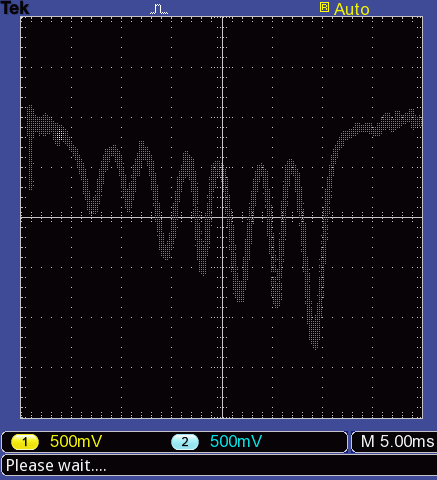
\includegraphics[width=\linewidth]{pictures/rb87-high-raw.png}
\caption{\textit{Quadratic Zeeman effect of $Rb^{87}$ at high RF power \\ }}
\justify

\subsubsection{$Rb^{85}$ quadratic Zeeman effect}
Now we consider the qudratic Zeeman effect of $Rb^{85}$. The settings are as 
follows.
\\
Detector amplifier gain = 20 \\
Mutiplier = 10 \\
$\nu$ = 4.1 MHz \\
Time constant = 100 ms \\
RF amplifier gain = 3 \\
Sweep time = 50 s \\
Horizontal Field current = 0.9872 A \\
RF amplitude = 1.0 V \\
\\
The data that was collected was the following.
\begin{minipage}{\linewidth}
\center
\begin{tabular}{|c|c|c|}
\hline
Peak & Amplitude (200 mV) & Voltage (V) \\ \hline
1 & 1.4 & 0.5060 \\ \hline
2 & 2.2 & 0.5460 \\ \hline
3 & 3.0 & 0.5839 \\ \hline
4 & 3.8 & 0.6228 \\ \hline
5 & 4.0 & 0.6604 \\ \hline
6 & 4.2 & 0.7002 \\ \hline
\end{tabular}
\captionof{table}{\textit{Data taken for low RF power quadratic Zeeman
effect \\}}
\label{tbl:10}
\end{minipage}
The plot of the data is shown on figure \ref{fig:26}. The screenshot of the 
osciloscope data is the following.
\center
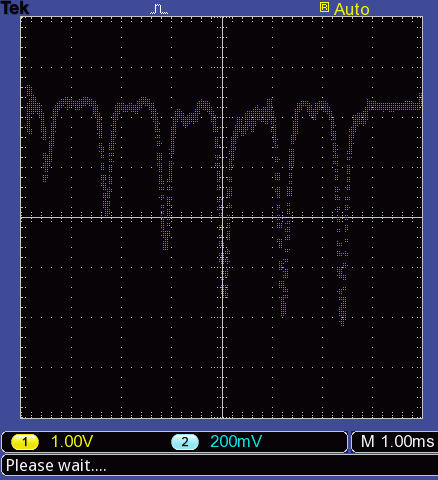
\includegraphics[width=\linewidth]{pictures/rb85-low-raw.png}
\caption{\textit{Quadratic Zeeman effect of $Rb^{85}$ at low RF power \\ }}
\justify
We will now consider the quadratic zeeman effect at high RF power.
\\
The settings used were the following.
\\
Detector amplifier gain = 20 \\
Mutiplier = 10 \\
$\nu$ = 4.1 MHz \\
Time constant = 100 ms \\
RF amplifier gain = 3 \\
Sweep time = 50 s \\
Horizontal Field current = 0.9872 A \\
RF amplitude = 2.5 V \\
\\
With the data collected being the following.
\begin{minipage}{\linewidth}
\center
\begin{tabular}{|c|c|c|}
\hline
Peak & Amplitude (200 mV) & Voltage (V) \\ \hline
1 & 1.8 & 0.5080 \\ \hline
2 & 1.8 & 0.5273 \\ \hline
3 & 2.6 & 0.5463 \\ \hline
4 & 3.2 & 0.5664 \\ \hline
5 & 3.0 & 0.5848 \\ \hline
6 & 4.2 & 0.6045 \\ \hline
7 & 3.6 & 0.6239 \\ \hline
8 & 5.0 & 0.6430 \\ \hline
9 & 4.5 & 0.6620 \\ \hline
10 & 5.0 & 0.6817 \\ \hline
11 & 5.0 & 0.7005 \\ \hline
\end{tabular}
\captionof{table}{\textit{Data taken for low RF power quadratic Zeeman
effect \\}}
\label{tbl:11}
\end{minipage}
The plot of the data is shown on figure \ref{fig:27}. The screenshot of the
osciloscope data is the following.
\center
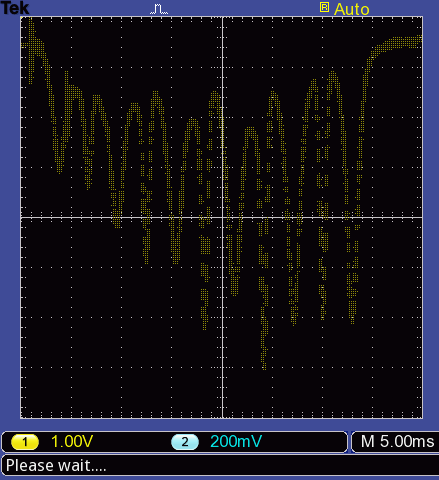
\includegraphics[width=\linewidth]{pictures/rb85-high-raw.png}
\caption{\textit{Quadratic Zeeman effect of $Rb^{85}$ at high RF power \\ }}
\justify

\subsection{Transient effects}
\begin{figure*}
\begin{minipage}[t]{\textwidth}
\center
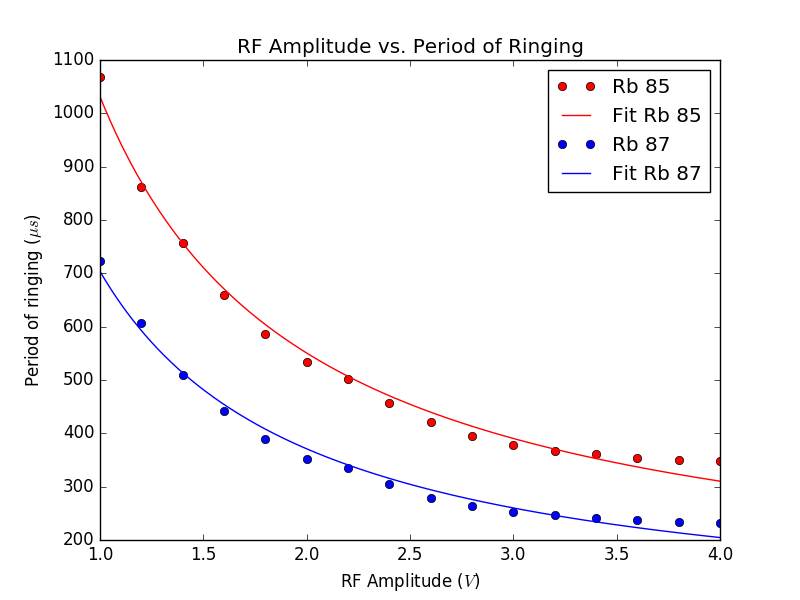
\includegraphics[width=0.45\linewidth]{pictures/per-rf.png}
\caption{\textit{Plot of the period of ringing in light intensity as a function 
of RF amplitude.}}
\label{fig:32}
\end{minipage}
\end{figure*}
For this part of the experiment we wanted to see what would happen where we to 
turn the RF magnetic field on and off quickly. Making pulses of RF magnetic 
fields. We first set the following parameters.
\\
\\
Detector amplifier gain = 1 \\
Mutiplier = 1 \\
$\nu$ = 100 kHz \\
Time constant = min. \\
RF amplifier gain = 8 \\
Sweep time = 50 s \\
Horizontal Field current = 3.68 mA \\
RF amplitude = 1.0 V \\
\\
We found that by plotting the incoming channels against time on the 
oscilloscope we got the following figure.
\center
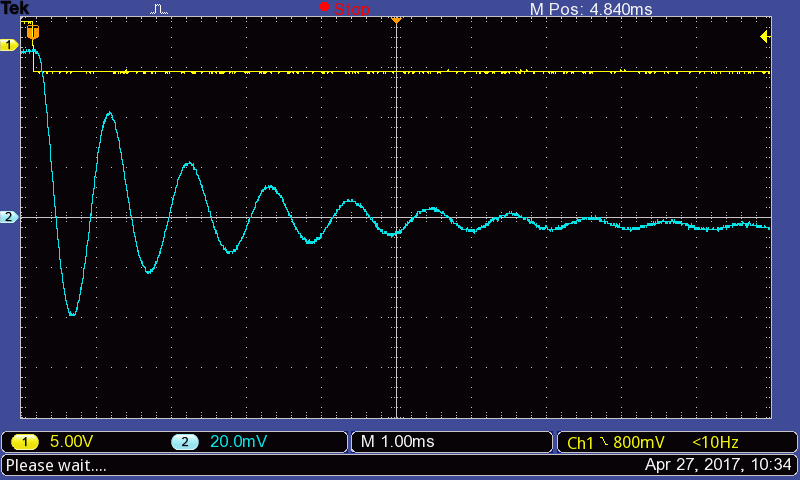
\includegraphics[width=\linewidth]{pictures/resonance-stuff.png}
\caption{\textit{Oscilations of the light intensity at 100 kHz and RF 
amplitude of 1.0 V. \\ }}
\justify
When we have the RF oscilate on and off at a frequency of 5 Hz we find that we 
get that picture when the RF is suddenly turned off. We did this for both of 
the isotopes of rubidium from RF amplitudes of 1.00 V to 4.00 V. When we looked 
for all the maxima in the figure and found the avreage period of oscilations 
we found that we got the following periods of oscilations.
\begin{minipage}{\linewidth}
\center
\begin{tabular}{|c|c|c|}
\hline
RF Amplitude & $Rb^{85}$ Period & $Rb^{87}$ Period \\ 
(V) & ($\mu$s) & ($\mu$s) \\ \hline
1.00 & 1067.2 & 723.0 \\ \hline
1.20 & 861.6 & 606.7 \\ \hline
1.40 & 757.0 & 508.8 \\ \hline
1.60 & 659.2 & 442.0 \\ \hline
1.80 & 586.0 & 390.0 \\ \hline
2.00 & 534.4 & 352.8 \\ \hline
2.20 & 501.3 & 334.4 \\ \hline
2.40 & 457.7 & 304.8 \\ \hline
2.60 & 421.7 & 279.3 \\ \hline
2.80 & 394.5 & 264.7 \\ \hline
3.00 & 377.5 & 252.7 \\ \hline
3.20 & 367.0 & 246.7 \\ \hline
3.40 & 360.5 & 240.7 \\ \hline
3.60 & 354.0 & 238.0 \\ \hline
3.80 & 350.9 & 233.3 \\ \hline
4.00 & 347.5 & 232.7 \\ \hline
\end{tabular}
\captionof{table}{Data that was used for figure \ref{fig:32} \\ }
\label{tbl:12}
\end{minipage}
The data for the RF amplitude on table \ref{tbl:12} was taken directly from the 
RF signal generator. The second column was gotten by reading through the data 
on each of the generated oscilation signals and finding the respective maxima. 
This was done by exporting the screenshot of the osciloscope to save all of the 
data files which includes two .CSV files for each of the signals. By using this 
we can get a much better estimate for the period as we do not have to manually 
do it and introduce human error due to inability to read difference in pixels.
\\
By fitting the plots to an equation that reads.
\begin{equation}
Y = \frac{A}{x} + B
\label{eqn:23}
\end{equation}
Where, x is the RF amplitude, Y the period of the ringing and the A, B 
parameters were calculated in Python with the curve fitting function to be.
\begin{minipage}{\linewidth}
\center
\begin{tabular}{|c|c|c|}
\hline
{} & A & B \\ \hline
$Rb^{85}$ & 960.0 $\pm$ 20.0 & 70.0 $\pm$ 10.0 \\ \hline
$Rb^{85}$ & 670.0 $\pm$ 20.0 & 38.0 $\pm$ 9.0 \\ \hline
\end{tabular}
\captionof{table}{\textit{Fit parameters to equation \ref{eqn:23} \\ }}
\label{tbl:13}
\end{minipage}
\\
Having calculated these values we were then able to find the ratio of the 
period of the ringing by dividing the A values. We found this value to be 1.44 
$\pm$ 0.05.
\\
When we compare this value to the expected value of 1.50 we believe to be 
sufficiently close to be able to take this value.



\begin{thebibliography}{9}
\bibitem{ref:1}
Bloom, A L (1960). Optical Pumping. \emph{Scientific American} October, 72.
\bibitem{ref:2}
Benumof, R (1965). Optical Pumping Theory and Experiments. \emph{American 
Journal of Physics 33}, 151.
\bibitem{ref:3}
UB 2015 Lab Manual. Optical Pumping.
\bibitem{ref:4}
Griffiths, D J (2005). Introduction to Quantum Mechanics. Upper Saddle river, 
New Jersey: \emph{Pearson Prentice Hall}.

\end{thebibliography}

\end{document}
